
\documentclass[preprint,12pt]{elsarticle}

\usepackage[spanish]{babel}
\usepackage{amssymb}
\usepackage{graphicx}
\usepackage{lineno}
\usepackage[utf8]{inputenc}
\usepackage{url}
\usepackage{natbib} 
\usepackage{amsmath} 
\usepackage{amssymb} 

\begin{document}
	
	\begin{frontmatter} 

		\title{\huge MESA DE AYUDA}
		
		\author{Huichi Contreras, Franklin Carlos            (2016056193)}
		\author{Gonzales Cave, Angel Gabriel                 (2017057861)}
		\author{Condori Quispe, Yhónn Joel	         	   (2016056358)} 
		\author{Pastor Mendoza, José Edilberto              (2016055237)} 
		\address{Escuela Profesional de Ingeniería de Sistemas}
		\address{Universidad Privada de Tacna}
		\address{Tacna, Perú}
		
%% ABSTRACT --------------------------------------------------------------------------------------------------------------------

		\begin{abstract}
The proposal the design a help desk for the technical support area of the Tacna Private University arises due to the demand of user requests to solve basic problems in their computer equipment, the general objective of this project is to provide the necessary information for the user and in turn provide the basic knowledge to solve technical problems in the equipment.Also, in order to expedite the optimal response of an incident, it is important to formalize the incident management process, in such a way that it adapts to the common requirements of the personnel, with the incidents being points of lost time and resources that the University or other organization would not like to waste.

		\end{abstract}

%% ----------------------------------------------------------------------------------------------------------------------------------

	\end{frontmatter}

%% RESUMEN ---------------------------------------------------------------------------------------------------------------------

\section{Resumen}
La propuesta de diseñar una mesa de ayuda para el área de soporte técnico de la Universidad Privada de Tacna surge debido a la demanda de solicitudes de los usuarios para resolver problemas básicos en sus equipos informáticos, el objetivo general de este proyecto es proporcionar la información necesaria para el usuario y a su vez proporcionan los conocimientos básicos para la resolución de problemas técnicos en el equipo.

Asimismo para poder agilizar la respuesta óptima de un incidente es importante la formalización del proceso de gestión de incidentes, de tal manera que se adecue a las exigencias comunes del personal , siendo los incidentes puntos de perdidas de tiempo y recursos que la Universidad o como otra organización no le gustaría desperdiciar.


%% ----------------------------------------------------------------------------------------------------------------------------------


%% INTRODUCION ----------------------------------------------------------------------------------------------------------------

\section{Introducción} 

El presente trabajo, estar enfocado a mejorar los tiempos de respuesta y la asistencia oportuna, permitiendo el desarrollo normal de actividades propias de los procesos de cada área.

Sabemos que hoy por hoy,  los equipos informáticos son herramientas indispensables en cualquier organización , ya que nos facilita la realización de distintas actividades laborales y que es necesario que estos equipos funcionen adecuamente durante todo el tiempo que se requiera en cualquier momento.

Para dar respuestas a incidentes ligados a los equipos informáticos o activos tanto de hardware y software cada activo ha sido en algún momento instalado , configurado o diseñado por una persona el cual será sindicado como el responsable para dar solución al problema en cuestión.

Es vital realizar un reconocimiento de soluciones al historial de problemas que se puedan sucitar en las diferentes áreas  para así encontrar la solución óptima y oportuna tanto en la infraestructura ya sean los equipos de cómputo y también en la asistencia a posibles fallas de estos elementos.

Este proyecto de implementación de una mesa de ayuda en el área de soporte técnico de la Universidad Privada de Tacna pretende garantizar la eficiencia y eficacia en el soporte y asistencia de consultas con la finalidad de  tener un  normal desarrollo de las actividades propias de la organización.

%% ----------------------------------------------------------------------------------------------------------------------------------


%% TITULO  ------------------------------------------------------------------------------------------------------------

\section{Título}

DISEÑO E IMPLEMENTACIÓN DE MESA DE AYUDA PARA EL ÁREA DE SOPORTE TÉCNICO DE LA UNIVERSIDAD PRIVADA DE TACNA

%% ----------------------------------------------------------------------------------------------------------------------------------

%% AUTORES  ------------------------------------------------------------------------------------------------------------

\section{Autores}

\begin{table}[htbp]
\begin{center}
\begin{tabular}{|l|l|}
\hline
Roles & Integrantes \\
\hline \hline
Product owner & Gonzales Cave, Angel Gabriel \\ \hline
Scrum master & Huichi Contreras, Franklin Carlos  \\ \hline
Equipo scrum & Condori Quispe, Yhónn Joel | Pastor Mendoza, José Edilberto \\ \hline
\end{tabular}
\caption{Integrantes del equipo}
\label{tabla:sencilla}
\end{center}
\end{table}



\begin{itemize}
\item Product owner : Es oficialmente responsable de gestionar el proyecto y de hacer visibles los Ìtems del Product Backlog. Toma las decisiones finales sobre los Ìtems del product backlog. Participa en la estimación de los Ìtems del backlog.
\item Scrum master: Es el responsable de llevar a cabo el proyecto de acuerdo a las reglas SCRUM, interactua con el equipo y los clientes y también es responsable de remover todo tipo de impedimento para el desarrollo. No asigna tareas a cada miembro del equipo ni toma decisiones para el equipo, los equipos son auto- organizativos. Hace mas de coach que de lider.
\item Equipo Scrum: Es el equipo del proyecto que tiene la autoridad para organizarse a sÌ mismo a fin de lograr los objetivos de cada sprint. Sus funciones son crear el sprint backlog, estimar los Ìtems del sprint backlog, revisar el product backlog y sugerir impedimentos para que estos se quiten del proyecto. 
\end{itemize}

%% ----------------------------------------------------------------------------------------------------------------------------------

%% PLANTEAMIENTO DEL PROBLEMA ------------------------------------------------------------------------------------------------------------

\section{Planteamiento del problema}
Actualmente los gestores de mesa de ayuda o el personal de soporte técnico de la Universidad Privada de Tacna tienen que proporcionar la misma información a los diferentes usuarios, puesto que existe redundancia en problemas de soporte técnico básicos a nivel de hardware y software que se presentan y muchas veces es difícil atender todas las peticiones al mismo instante; lo cual demanda pérdida de tiempo en la solución de dichos problemas. A su vez las empresas  cuentan con una sola persona encargada de dar el soporte técnico que solicita el personal, dado que al existir demanda de problemas técnicos, la persona encargada tenga que atender los problemas presentados en el orden que lo asistieron, dejando al resto del personal en espera. El tiempo que demora el encargado de dar el soporte técnico a cada problema del personal, impide que el mismo pueda realizar el resto de sus actividades diarias, pues muchas veces el encargado de dar el soporte técnico al personal también es encargado de otras actividades de la empresa. 

%%  SUBSECCION 

\subsection {\textbf{Problema}}
Demora en solución de problemas de soporte tecnico a nivel de software y hardware. Suele suceder que los componentes de cómputo funcionen de forma incorrecta que causa un desempeño poco fiable del sistema, futuros fallos en el equipo y poca garantia en el servicio de la empresa. La carencia de una herramienta informática que facilite la rápida obtención de reportes que contengan los indicadores de desempeño de la Gestión de Incidencias en la Mesa de Ayuda de la Universidad Privada de Tacna ocasionando que esta falta de información oportuna no brinde el soporte a la Toma de Decisiones sobre las estrategias de Atención en la Gestión de Incidencias.

%%  SUBSECCION 

\subsection {\textbf{Justificacion}}

Las áreas de la Universidad Privada de Tacna en general vienen realizando diversas y diferentes tareas que estan ligadas a los procesos academicos y administrativos y también a la mejora continua de su imagen institucional.
En cumplimiento a sus funciones la Oficina de Soporte Técnico debe garantizar en todo momento de manera óptima la prestación de un servicio de calidad para continuar con las actividades en caso de la generación de para que el personal pueda ejecutar sus funciones.
 
Es necesario concentrar por medio de una mesa de ayuda, la atención de las solicitudes relacionadas con el hardware  software teniendo un inventario de equipos de cómputo actualizado, brindando soluciones a las solicitudes generadas por los usuarios, facilitando así una atención rápida y oportuna, garantizando la continuidad de las actividades del personal.

Con este servicio los usuarios podrán aclarar sus dudas y solucionar problemas ténicos basicos.

Ya no pasarán mucho tiempo esperando para que un ténico solucione los problemas, los clientes tendran un servicio a la vanguardia de la tecnologia y de esta manera la perdida de tiempo, las consultas repetitivas podran solventarse en menos tiempo.

Este servicio permitirá a su vez ir capacitando el conocimiento del usuario en soporte técnico de hardware y software; cuando vuelva a tener el mismo inconveniente con su equipo segurirá las pautas que le proporciono el sistema, evitando llamar al encargado de dar soporte a los usuarios y de esta manera el tiempo que se pierde tanto del encargado de dar soporte como del usuario quedará reducido.

El sistema no solo beneficiara al gestor de mesa de ayuda encargado del soporte tecnico sino tambien al usuario y al avance de las empresas, puesto que mientras menos tiempo se demande en resolver los problemas a nivel básico de soporte técnico en los equipos, más tiempo tiene el usuario de seguir trabajando en la actividad de la empresa.


%%  SUBSECCION 

\subsection {\textbf{Alcance}}
El propósito de este proyecto es desarrollar un sistema de mesa de ayuda; este servicio permitira que el usuario obtenga la informacion que necesita para resolver algún inconveniente que se le presente, sin la necesidad de capacitarse en soporte técnico básico.

El sistema de mesa de ayuda permitirá que el tiempo en resolución de problemas técnicos sean resueltos a la brevedad posible por el usuario puesto que contara con un entorno que dispondra con las preguntas o problemas mas frecuentes, en caso sea necesario se solicitará la informacion del técnico de la empresa.

%% ----------------------------------------------------------------------------------------------------------------------------------

%% OBJETIVOS ------------------------------------------------------------------------------------------------------------

%%  SUBSECCION 

\subsection{\textbf{General}}

Desarrollar un servicio de mesa de ayuda para la Universidad Privada de tacna con el fin de informar al usuario en los problemas mas frecuentes, mediante el uso de herramientas informáticas.

%%  SUBSECCION 

\subsection{\textbf{Especificos}}

\begin{itemize}

\item Analizar cuáles son las peticiones de soporte técnico mas solicitadas por los usuarios, para obtener la informacion necesaria y definir los requerimientos para el correcto desarrollo del sistema
\item Mejorar la productivdad de la empresa informando a los usuarios sobre como solucionar los problemas comunes.
\end{itemize}


%% ----------------------------------------------------------------------------------------------------------------------------------
 

%% REFERENTES TEORICOS ---------------------------------------------------------------------------------------------------

\section{Referentes Teoricos}
Biblioteca de Infraestructura de Tecnologías de la Información (ITIL) : Es un marco de buenas prácticas y conceptos para la gestión de servicios de tecnologías de la información, el desarrollo de tecnologías de la información y las operaciones relacionadas con diversas áreas de servicios TI.

A continuación se describe la conformación actual de ITIL v3 :
\begin{itemize}
\item Libro 1  Estrategia del Servicio 
Propone tratar la gestión de servicios no sólo como una capacidad sino como un activo estratégico
\item Libro 2 Diseño del Servicio
Cubre los principios y métodos necesarios para transformar los objetivos estratégicos en portafolios de servicios y activos.
\item Libro 3 Transición del Servicio
Cubre el proceso de transición para la implementación de nuevos servicios o su mejora
\item Libro 4 Operación del Servicio
Cubre las mejores prácticas para la gestión del día a día en la operación del servicio.
\item Libro 5 Mejora Continua del Servicio
Proporciona una guía para la creación y mantenimiento del valor ofrecido a los clientes a través de un diseño, transición y operación del servicio optimizado.
\end{itemize}
ITIL es un marco de referencia de las buenas prácticas, las que permiten incorporar estándares en los procesos, métodos y actividades existentes orientadas a un entorno de calidad en gestión de servicios TI, para satisafacer las necesidades y requerimientos de los clientes.

%% ----------------------------------------------------------------------------------------------------------------------------------


%% DESARROLLO DE LA PROPUESTA ---------------------------------------------------------------------------------------------------

\section{Desarrollo de la propuesta}

EDITAR\\

%%  SUBSECCION 

\subsection{\textbf{Tecnología de información}}

\begin{itemize}
\item Python es un lenguaje de programación interpretado cuya filosofía hace hincapié en una sintaxis que favorezca un código legible. Se trata de un lenguaje de programación multiparadigma, ya que soporta orientación a objetos, programación imperativa y, en menor medida, programación funcional. Es un lenguaje interpretado, dinámico y multiplataforma.

\item Flask es un framework minimalista escrito en Python que permite crear aplicaciones web rápidamente y con un mínimo número de líneas de código.

\item Microsoft SQL Server es un sistema de gestión de base de datos relacional, desarrollado por la empresa Microsoft.
\end{itemize}

%%  SUBSECCION 

\subsection{\textbf{Metodología, técnicas usadas}}

SCRUM es una metodologÌa para gestion, mejora y mantenimiento de un sistema nuevo o existente. SCRUM se concentra en como los miembros del equipo deberÌan funcionar a fin de producir un sistema flexible en un entorno que cambia constantemente. \cite{ScrumDef}

\subsubsection{\textbf{Inicio}}

\begin{itemize}
\item Planeamiento: Consiste en establecer la visión, el presupuesto, forma de financiamiento y el backlog del producto. En esta fase se selecciona que funcionalidad es la mas apropiada para desarrollo inmediato. Tambien se establece el equipo de trabajo, se evaluan las herramientas de desarrollo y se define la fecha de entrega (es una fecha aproximada). \cite{ScrumDef}

\item Arquitectura : Esta fase consiste en la conceptualización y análisis. Si el proyecto se trata de la mejora de un nuevo sistema, sólo se realiza un analisis limitado. Se realiza un diseño de alto nivel para actualizar los modelos del dominio y reflejar el contexto del nuevo sistema y los requerimientos y las modificaciones necesarias de la arquitectura del sistema. Los diseñadores y arquitectos dividen el proyecto en paquetes basandose en los Ìtems del backlog. En la jerga de SCRUM se llaman ìpaquetesî a los objetos o componentes que necesitan cambiarse en cada iteración. \cite{ScrumDef}
\end{itemize}

\subsubsection{\textbf{Desarrollo}}
En esta etapa se realiza el desarrollo propiamente dicho. También se la conoce como ìIngenierÌa concurrenteî. La misma se divide en iteraciones que proveen como resultado funcionalidades incrementales al fin de cada una de ellas. Dichas iteraciones se llaman sprints. \\
Un sprint dura aproximadamente entre una semana y 30 dÌas. Cada sprint incluye las fases tradicionales del desarrollo de software: requerimientos, an·lisis, diseño, desarrollo y entrega.
Durante un sprint no se utilizan diagramas de gantt para seguimiento de tareas (estos parten del supuesto que las tareas de un proyecto se pueden identificar y ordenar), debido a que el desarrollo es semi-caotico y cambiante como para que se le aplique un proceso definido. \\
Durante un sprint no se pueden cambiar los miembros del equipo scrum. Tampoco pueden introducirse cambios durante un sprint (si surge algun cambio se incluira en el backlog del producto, pero no en el del sprint). \\
El scrum master mantiene el sprint backlog. Actualiza las tareas finalizadas y para las que no lo estan, el tiempo que el equipo piensa que tomara para terminarlas. \cite{ScrumDef} \\

\subsubsection{\textbf{Reuniones Scrum}}
Durante un sprint, todos los dÌas se realizan reuniones llamadas ìSCRUMî. El objetivo de las mismas es quitar los impedimentos que le surgen a los miembros del equipo scrum. Cada una de ellas dura aproximadamente 15 minutos. A cada miembro del equipo scrum se le pregunta:
\begin{itemize}
\item ¿Qué hizo durante las ultimas 24 horas?
\item ¿Qué planea hacer las proximas 24 horas?
\item ¿Qué obstaculos se le han presentado en las últimas 24 horas ?
\end{itemize}
Estas reuniones deben realizarse obligatoriamente.\cite{ScrumDef}

\subsubsection{\textbf{Cierre}}
Esta etapa comienza cuando el equipo de management decide que las variables de entorno, tales como los requerimientos se han completado. En esta etapa se genera la documentaciÛn final, se realiza el testing pre-lanzamiento y el lanzamiento propiamente dicho. \cite{ScrumDef}

\begin{figure}[htb]
	\begin{center}
		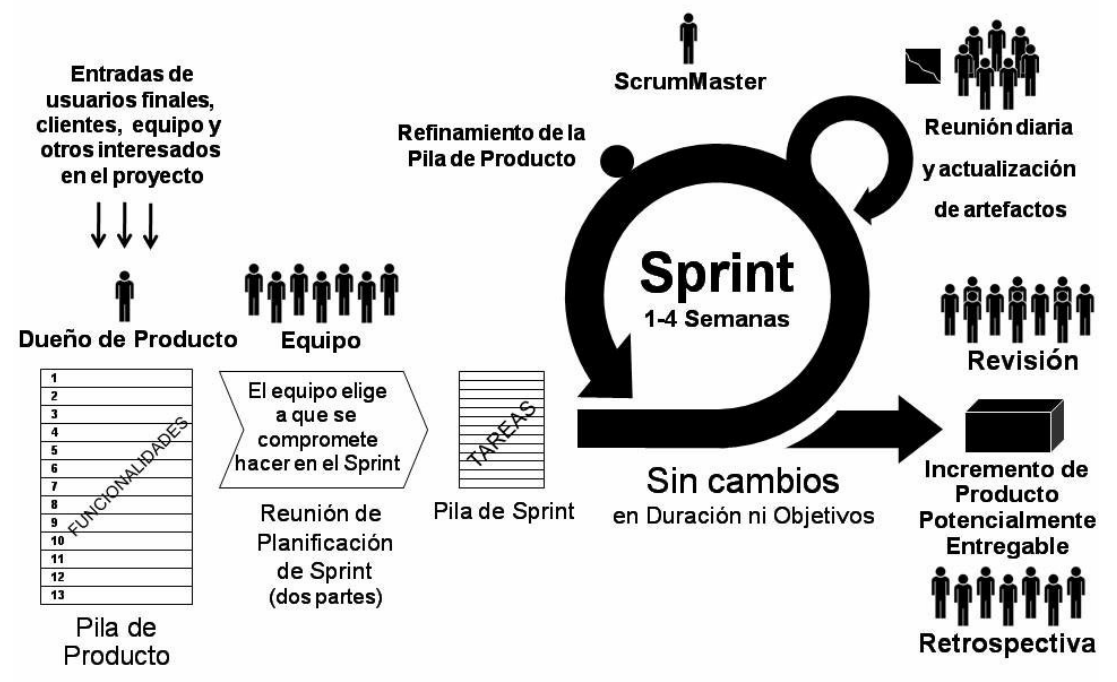
\includegraphics[width=14cm]{./IMAGENES/Scrum} 
		\caption{Cronograma del proyecto}
	\end{center}
\end{figure}


%% ----------------------------------------------------------------------------------------------------------------------------------

%% CRONOGRAMA (PERSONAS, TIEMPO, OTROS RECURSOS) ---------------------------------------------------------------------------------------------------

\section{Cronograma}

\begin{figure}[htb]
	\begin{center}
		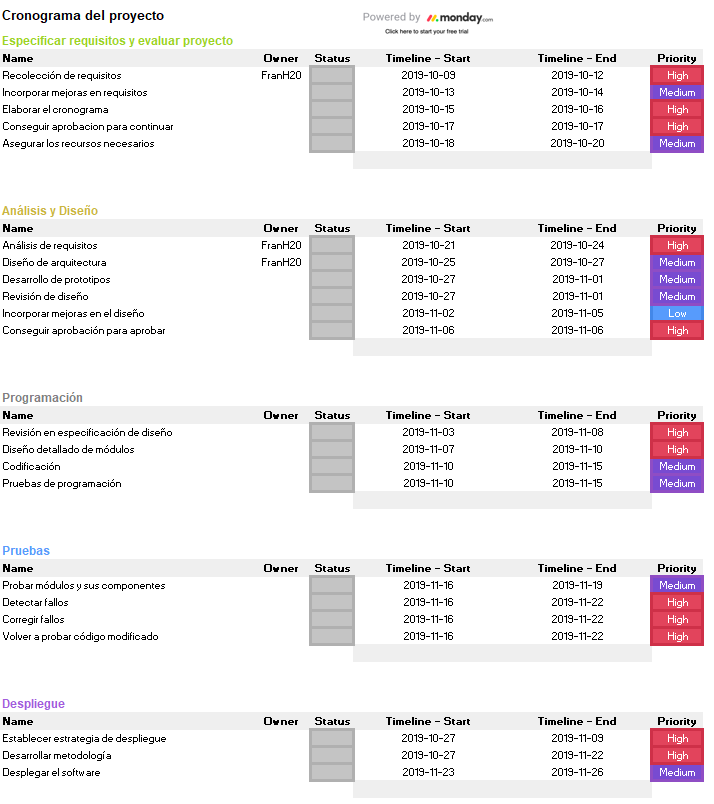
\includegraphics[width=14cm]{./IMAGENES/Gannt} 
		\caption{Cronograma del proyecto}
	\end{center}
\end{figure}

%% ----------------------------------------------------------------------------------------------------------------------------------



%%  REFERENCIAS BIBLIOGRÁFICAS  (OJO NO TOCAR CON CITEP SOLO SE PONEN)------------------------------------------------------------------------------------------
	
	\newpage
	
	\bibliographystyle{apalike} 	%ESTILO
	\bibliography{BIBLIOGRAFIA}	 
	
	
\end{document}
